 \documentclass[answers]{exam}
\newif\ifanswers
\answerstrue % comment out to hide answers

\usepackage{lastpage} % Required to determine the last page for the footer
\usepackage{extramarks} % Required for headers and footers
\usepackage[usenames,dvipsnames]{color} % Required for custom colors
\usepackage{graphicx} % Required to insert images
\usepackage{listings} % Required for insertion of code
\usepackage{courier} % Required for the courier font
\usepackage{lipsum} % Used for inserting dummy 'Lorem ipsum' text into the template
\usepackage{enumerate}
\usepackage{subfigure}
\usepackage{booktabs}
\usepackage{amsmath, amsthm, amssymb}
\usepackage{hyperref}
\usepackage{datetime}
\usepackage{minted}
\settimeformat{ampmtime}
\usepackage{algpseudocode}
\usepackage{algorithmicx}
\usepackage[ruled]{algorithm}
\usepackage{tikz-dependency}

\usepackage{tikz}
\usetikzlibrary{positioning,patterns,fit,calc}
% Margins
\topmargin=-0.45in
\evensidemargin=0in
\oddsidemargin=0in
\textwidth=6.5in
\textheight=9.0in
\headsep=0.25in

\linespread{1.1} % Line spacing

% Set up the header and footer
%\pagestyle{fancy}
%\rhead{\hmwkAuthorName} % Top left header
%\lhead{\hmwkClass: \hmwkTitle} % Top center head
%\lfoot{\lastxmark} % Bottom left footer
%\cfoot{} % Bottom center footer
%\rfoot{Page\ \thepage\ of\ \protect\pageref{LastPage}} % Bottom right footer
%\renewcommand\headrulewidth{0.4pt} % Size of the header rule
%\renewcommand\footrulewidth{0.4pt} % Size of the footer rule

\pagestyle{headandfoot}
\runningheadrule{}
\firstpageheader{CS 224n}{Assignment 3}{}
\runningheader{CS 224n} {Assignment 3} {Page \thepage\ of \numpages}
\firstpagefooter{}{}{} \runningfooter{}{}{}

\setlength\parindent{0pt} % Removes all indentation from paragraphs

%----------------------------------------------------------------------------------------
%	CODE INCLUSION CONFIGURATION
%----------------------------------------------------------------------------------------

\definecolor{MyDarkGreen}{rgb}{0.0,0.4,0.0} % This is the color used for comments
\lstloadlanguages{Python} % Load Perl syntax for listings, for a list of other languages supported see: ftp://ftp.tex.ac.uk/tex-archive/macros/latex/contrib/listings/listings.pdf
\lstset{language=Python, % Use Perl in this example
        frame=single, % Single frame around code
        basicstyle=\footnotesize\ttfamily, % Use small true type font
        keywordstyle=[1]\color{Blue}\bf, % Perl functions bold and blue
        keywordstyle=[2]\color{Purple}, % Perl function arguments purple
        keywordstyle=[3]\color{Blue}\underbar, % Custom functions underlined and blue
        identifierstyle=, % Nothing special about identifiers
        commentstyle=\usefont{T1}{pcr}{m}{sl}\color{MyDarkGreen}\small, % Comments small dark green courier font
        stringstyle=\color{Purple}, % Strings are purple
        showstringspaces=false, % Don't put marks in string spaces
        tabsize=5, % 5 spaces per tab
        %
        % Put standard Perl functions not included in the default language here
        morekeywords={rand},
        %
        % Put Perl function parameters here
        morekeywords=[2]{on, off, interp},
        %
        % Put user defined functions here
        morekeywords=[3]{test},
       	%
        morecomment=[l][\color{Blue}]{...}, % Line continuation (...) like blue comment
        numbers=left, % Line numbers on left
        firstnumber=1, % Line numbers start with line 1
        numberstyle=\tiny\color{Blue}, % Line numbers are blue and small
        stepnumber=5 % Line numbers go in steps of 5
}

%----------------------------------------------------------------------------------------
%	NAME AND CLASS SECTION
%----------------------------------------------------------------------------------------

\newcommand{\hmwkTitle}{Dependency Parsing} % Assignment title
\newcommand{\hmwkClass}{CS\ 224n Assignment \#3} % Course/class
\newcommand{\ifans}[1]{\ifanswers \color{red} \textbf{Solution: } #1 \color{black} \fi}

% \newcommand{\ifans}[1]{}

\input macros.tex
\input std_macros.tex

%----------------------------------------------------------------------------------------
%	TITLE PAGE
%----------------------------------------------------------------------------------------
\qformat{\Large\bfseries\thequestion{}. \thequestiontitle{} (\thepoints{})\hfill}

\title{
\vspace{-1in}
\textmd{\textbf{\hmwkClass:\ \hmwkTitle}}
}
\author{}
%\date{\textit{\small Updated \today\ at \currenttime}} % Insert date here if you want it to appear below your name
\date{}

\setcounter{section}{0} % one-indexing
\begin{document}

\maketitle
% \vspace{-10pt}

In this assignment, you will build a neural dependency parser using PyTorch. For a review of the fundamentals of PyTorch, please check out the PyTorch review session on Canvas.  In Part 1, you will learn about two general neural network techniques (Adam Optimization and Dropout). In Part 2, you will implement and train a dependency parser using the techniques from Part 1, before analyzing a few erroneous dependency parses.

Please tag the questions correctly on Gradescope, the TAs  will take points off if you don't tag questions. 
\begin{questions}
    \graphicspath{ {images/} }

% real numbers R symbol
\newcommand{\Real}{\mathbb{R}}

% encoder hidden
\newcommand{\henc}{\bh^{\text{enc}}}
\newcommand{\hencfw}[1]{\overrightarrow{\henc_{#1}}}
\newcommand{\hencbw}[1]{\overleftarrow{\henc_{#1}}}

% encoder cell
\newcommand{\cenc}{\bc^{\text{enc}}}
\newcommand{\cencfw}[1]{\overrightarrow{\cenc_{#1}}}
\newcommand{\cencbw}[1]{\overleftarrow{\cenc_{#1}}}

% decoder hidden
\newcommand{\hdec}{\bh^{\text{dec}}}

% decoder cell
\newcommand{\cdec}{\bc^{\text{dec}}}

\titledquestion{Neural Machine Translation with RNNs}[45]
 In Machine Translation, our goal is to convert a sentence from the \textit{source} language (e.g. Mandarin Chinese) to the \textit{target} language (e.g. English). In this assignment, we will implement a sequence-to-sequence (Seq2Seq) network with attention, to build a Neural Machine Translation (NMT) system. In this section, we describe the \textbf{training procedure} for the proposed NMT system, which uses a Bidirectional LSTM Encoder and a Unidirectional LSTM Decoder.\newline

\begin{figure}[h]
    \begin{center}
        \captionsetup{width=0.8\textwidth}
        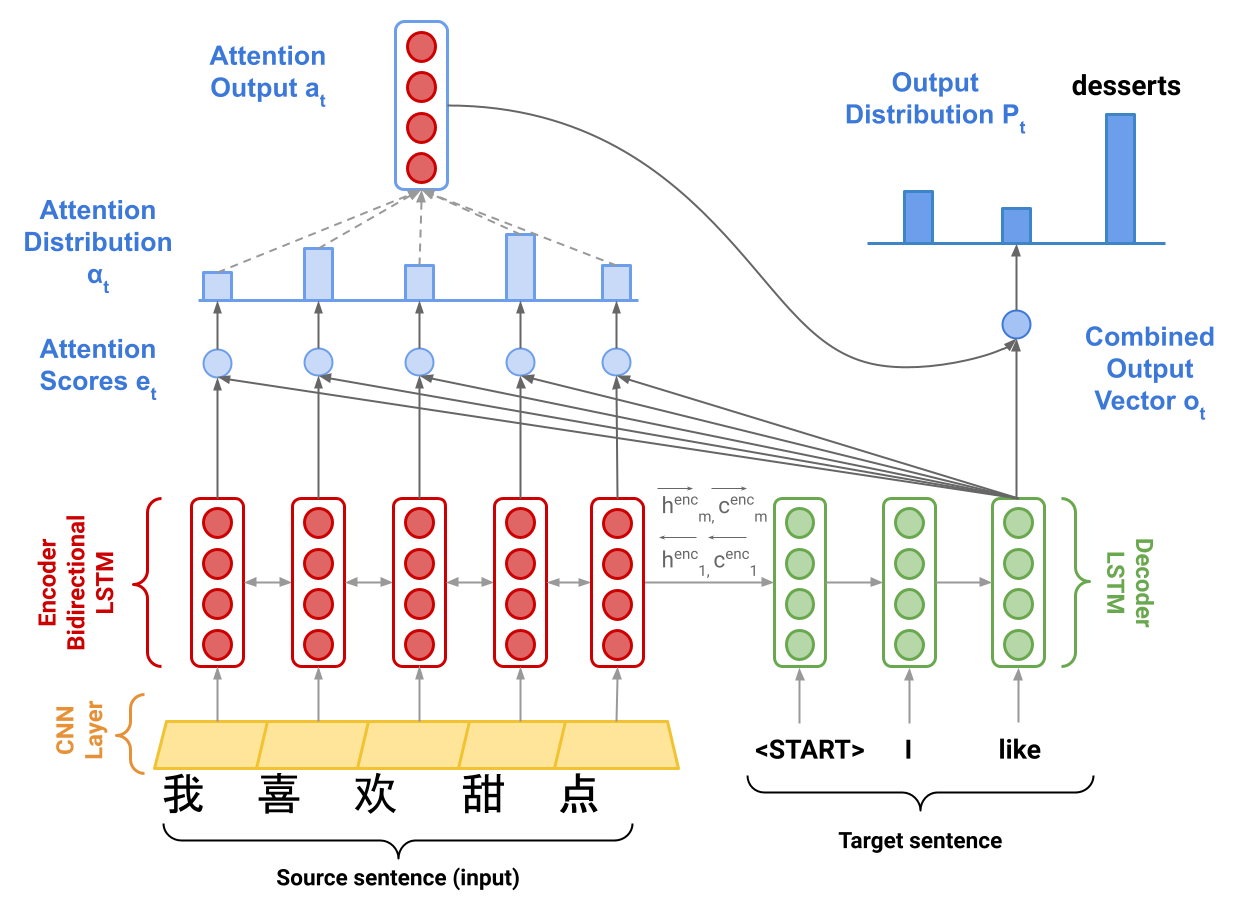
\includegraphics[width=0.8\textwidth]{images/Assignment 4 Figure.png}
        \caption{Seq2Seq Model with Multiplicative Attention, shown on the third step of the decoder. Hidden states $\henc_i$ and cell states $\cenc_i$ are defined on the next page.
        }
        \label{nmt-figure}
    \end{center}
\end{figure}

\subsection*{Model description (training procedure)}
 Given a sentence in the source language, we look up the character or word embeddings from an \textbf{embeddings matrix}, yielding $\bx_1, \dots, \bx_m$ ($\bx_i \in \Real^{e \times 1}$), where $m$ is the length of the source sentence and $e$ is the embedding size. We then feed the embeddings to a \textbf{convolutional layer} \footnote{Checkout \url{https://cs231n.github.io/convolutional-networks} for an in-depth description for convolutional layers if you are not familiar} while maintaining their shapes. We feed the convolutional layer outputs to the \textbf{bidirectional encoder}, yielding hidden states and cell states for both the forwards ($\rightarrow$) and backwards ($\leftarrow$) LSTMs. The forwards and backwards versions are concatenated to give hidden states $\henc_i$ and cell states $\cenc_i$:
 
\begin{align}
    \henc_i = [\hencbw{i}; \hencfw{i}] \enspace &\text{where}\enspace \henc_i \in \Real^{2h \times 1}, \hencbw{i}, \hencfw{i} \in \Real^{h \times 1} &1 \le i \le m \\
    \cenc_i = [\cencbw{i}; \cencfw{i}] \enspace &\text{where} \enspace \cenc_i \in \Real^{2h \times 1}, \cencbw{i}, \cencfw{i} \in \Real^{h \times 1} &1 \le i \le m
\end{align}

We then initialize the \textbf{decoder}'s first hidden state $\hdec_0$ and cell state $\cdec_0$ with a linear projection of the encoder's final hidden state and final cell state.\footnote{If it's not obvious, think about why we regard $[\hencbw{1}, \hencfw{m}]$ as the `final hidden state' of the Encoder.} 

\begin{align}
    \hdec_0 = \bW_{h}[\hencbw{1}; \hencfw{m}] \enspace &\text{where} \enspace \hdec_0 \in \Real^{h \times 1}, \bW_{h} \in \Real^{h \times 2h}\\
    \cdec_0 = \bW_{c}[\cencbw{1}; \cencfw{m}] \enspace &\text{where} \enspace \cdec_0 \in \Real^{h \times 1}, \bW_{c} \in \Real^{h \times 2h}
\end{align}

With the decoder initialized, we must now feed it a target sentence. On the $t^{th}$ step, we look up the embedding for the $t^{th}$ subword,  $\by_t \in \Real^{e \times 1}$. We then concatenate $\by_t$ with the \textit{combined-output vector} $\bo_{t-1} \in \Real^{h \times 1}$ from the previous timestep (we will explain what this is later down this page!\@) to produce $\overline{\by_t} \in \Real^{(e+h) \times 1}$. Note that for the first target subword (i.e. the start token) $\bo_{0}$ is a zero-vector. We then feed $\overline{\by_t}$ as input to the decoder. 

\begin{align}
    \hdec_t, \cdec_t = \text{Decoder}(\overline{\by_t}, \hdec_{t-1}, \cdec_{t-1}) \enspace &\text{where} \enspace \hdec_t \in \Real^{h \times 1}, \cdec_t \in \Real^{h \times 1}\\
\end{align}

We then use $\hdec_t$ to compute  multiplicative attention over $\henc_1, \dots, \henc_m$:

\begin{align}
    \be_{t, i} = (\hdec_t)^T\bW_{\text{attProj}}\henc_i \enspace &\text{where} \enspace \be_{t} \in \Real^{m \times 1}, \bW_{\text{attProj}}\in \Real^{h \times 2h} & 1 \le i \le m \\
    \alpha_t= \text{softmax}(\be_t) \enspace &\text{where} \enspace \alpha_t \in \Real^{m \times 1}\\
    \ba_t = \sum_{i=1}^{m}\alpha_{t,i}\henc_i \enspace &\text{where} \enspace \ba_t \in \Real^{2h \times 1}
\end{align}
 
$\be_{t, i}$ is a scalar, the $i$th element of $\be_{t} \in \Real^{m \times 1}$, computed using the hidden state of the decoder at the $t$th step, $\hdec_t \in \Real^{h \times 1}$, the attention projection $\bW_{\text{attProj}} \in \Real^{h \times 2h}$, and the hidden state of the encoder at the $i$th step, $\henc_i \in \Real^{2h \times 1}$.

We now concatenate the attention output $\ba_t$ with the decoder hidden state $\hdec_t$ and pass this through a linear layer, tanh, and dropout to attain the \textit{combined-output} vector $\bo_{t}$.

\begin{align}   
    \bu_{t} = [\ba_{t}; \hdec_t] \enspace &\text{where} \enspace \bu_t \in  \Real^{3h \times 1} \\
    \bv_t = \bW_{u}\bu_t \enspace &\text{where} \enspace \bv_t \in \Real^{h \times 1}, \bW_{u} \in \Real^{h \times 3h}\\
    \bo_t = \text{dropout}(\text{tanh}(\bv_t)) \enspace &\text{where} \enspace \bo_t \in \Real^{h \times 1}
\end{align}

Then, we produce a probability distribution $\bP_t$ over target subwords at the $t^{th}$ timestep:

\begin{align}
    \bP_t = \text{softmax}(\bW_{\text{vocab}}\bo_{t}) \enspace &\text{where} \enspace \bP_t \in \Real^{V_{t} \times 1}, \bW_{\text{vocab}} \in \Real^{V_{t} \times h}
\end{align}

Here, $V_{t}$ is the size of the target vocabulary. Finally, to train the network we then compute the cross entropy loss between $\bP_t$ and $\bg_{t}$, where $\bg_{t}$ is the one-hot vector of the target subword at timestep $t$:

\begin{align}
    J_t(\theta) = \mathrm{CrossEntropy}(\bP_t,\bg_{t})
\end{align}

Here, $\theta$ represents all the parameters of the model and $J_t(\theta)$ is the loss on step $t$ of the decoder.
Now that we have described the model, let's try implementing it for Mandarin Chinese to English translation!

\subsection*{Setting up your Virtual Machine}
Follow the instructions in the \href{https://docs.google.com/document/d/11kRyfClhTi4-MC1feWWCMI31fHpTzddASsDa48_Dd9E/edit?usp=sharing}{CS224n Azure Guide} (link also provided on website and Ed) in order to create your VM instance. This should take you approximately 45 minutes. Though you will need the GPU to train your model, we strongly advise that you first develop the code locally and ensure that it runs, before attempting to train it on your VM. GPU time is expensive and limited. It takes approximately \textbf{1.5 to 2 hours} to train the NMT system. We don't want you to accidentally use all your GPU time for debugging your model rather than training and evaluating it. Finally, \textbf{make sure that your VM is turned off whenever you are not using it.}

\textbf{\textcolor{red}{If your Azure subscription runs out of money, your VM will be temporarily locked and inaccessible. If that happens, please fill out a request form \href{https://forms.gle/PUwiA1rR5aQNWxYt6}{here}.}}

In order to run the model code on your \textbf{local} machine, please run the following command to create the proper virtual environment:

\begin{lstlisting}
    conda env create --file local_env.yml
\end{lstlisting}

Note that this virtual environment \textbf{will not} be needed on the VM.\newline

\subsection*{Implementation and written questions}

\begin{parts}
    \part [2] (coding) In order to apply tensor operations, we must ensure that the sentences in a given batch are of the same length. Thus, we must identify the longest sentence in a batch and pad others to be the same length. Implement the \texttt{pad\_sents} function in \texttt{utils.py}, which shall produce these padded sentences.
    
    \part[3] (coding) Implement the \texttt{\_\_init\_\_} function in \texttt{model\_embeddings.py} to initialize the necessary source and target embeddings.

    \part[4] (coding) Implement the \texttt{\_\_init\_\_} function in \texttt{nmt\_model.py} to initialize the necessary model layers (LSTM, CNN, projection, and dropout) for the NMT system.
    
    \part[8] (coding) Implement the \texttt{encode} function in \texttt{nmt\_model.py}. This function converts the padded source sentences into the tensor $\bX$, generates $\henc_1, \dots, \henc_m$, and computes the initial state $\hdec_0$ and initial cell $\cdec_0$ for the Decoder. You can run a non-comprehensive sanity check by executing:
    
\begin{lstlisting}
    python sanity_check.py 1d
\end{lstlisting}
    
    \part[8] (coding) Implement the \texttt{decode} function in \texttt{nmt\_model.py}. This function constructs $\bar{\by}$ and runs the \texttt{step} function over every timestep for the input. You can run a non-comprehensive sanity check by executing:

     
\begin{lstlisting}
    python sanity_check.py 1e
\end{lstlisting}
    
    \part[10] (coding) Implement the \texttt{step} function in \texttt{nmt\_model.py}. This function applies the Decoder's LSTM cell for a single timestep, computing the encoding of the target subword $\hdec_t$, the attention scores $\be_t$, attention distribution $\alpha_t$, the attention output $\ba_{t}$, and finally the combined output $\bo_t$. You can run a non-comprehensive sanity check by executing:
    
    
\begin{lstlisting}
    python sanity_check.py 1f
\end{lstlisting}
           
    
    \part [3] (written) The \texttt{generate\_sent\_masks()} function in \texttt{nmt\_model.py} produces a tensor called \texttt{enc\_masks}. It has shape (batch size, max source sentence length) and contains 1s in positions corresponding to `pad' tokens in the input, and 0s for non-pad tokens. Look at how the masks are used during the attention computation in the \texttt{step()} function (lines 311-312). 
    
    First explain (in around three sentences) what effect the masks have on the entire attention computation.
    Then explain (in one or two sentences) why it is necessary to use the masks in this way.

    \ifans{}
\end{parts}

Now it's time to get things running! As noted earlier, we recommend that you develop the code on your personal computer.  Confirm that you are running in the proper conda environment and then execute the following command to train the model on your local machine:
    
\begin{lstlisting}
    sh run.sh train_local
    (Windows) run.bat train_local
\end{lstlisting}

For a faster way to debug by training on less data, you can run the following instead:
\begin{lstlisting}
    sh run.sh train_debug
    (Windows) run.bat debug
\end{lstlisting}


To help with monitoring and debugging, the starter code uses tensorboard to log loss and perplexity during training using TensorBoard\footnote{https://pytorch.org/docs/stable/tensorboard.html}. TensorBoard provides tools for logging and visualizing training information from experiments. To open TensorBoard, run the following in your conda environment:

\begin{lstlisting}
   tensorboard --logdir=runs
\end{lstlisting}

You should see a significant decrease in loss during the initial iterations. Once you have ensured that your code does not crash (i.e. let it run till \texttt{iter 10} or \texttt{iter 20}), power on your VM from the Azure Web Portal. Then read the \textit{Managing Code Deployment to a VM} section of our \href{https://docs.google.com/document/d/11kRyfClhTi4-MC1feWWCMI31fHpTzddASsDa48_Dd9E/edit?usp=sharing}{Practical Guide to VMs} (link also given on website and Ed) for instructions on how to upload your code to the VM.

Next, install necessary packages to your VM by running:
    
\begin{lstlisting}
    pip install -r gpu_requirements.txt
\end{lstlisting}

Finally, turn to the \textit{Managing Processes on a VM} section of the Practical Guide and follow the instructions to create a new tmux session. Concretely, run the following command to create tmux session called \texttt{nmt}. 
\begin{lstlisting}
    tmux new -s nmt
\end{lstlisting}


Once your VM is configured and you are in a tmux session, execute:
\begin{lstlisting}
    sh run.sh train
    (Windows) run.bat train
\end{lstlisting}
    
Once you know your code is running properly, you can detach from session and close your ssh connection to the server. To detach from the session, run:
\begin{lstlisting}
    tmux detach
\end{lstlisting}
    
You can return to your training model by ssh-ing back into the server and attaching to the tmux session by running:
    
\begin{lstlisting}
    tmux a -t nmt
\end{lstlisting}

\begin{parts}
\setcounter{partno}{7}
\part[3] (written) Once your model is done training (\textbf{this should take under 2 hours on the VM}), execute the following command to test the model:
\begin{lstlisting}
sh run.sh test
(Windows) run.bat test
\end{lstlisting}
    Please report the model's corpus BLEU Score. It should be larger than 18.
    
    \ifans{}
    
    \part[4] (written) In class, we learned about dot product attention, multiplicative attention, and additive attention.  As a reminder, dot product attention is $\be_{t,i} = \bs_t^T\bh_i$, multiplicative attention is $\be_{t,i} = \bs_t^T\bW\bh_i$, and additive attention is $\be_{t,i} = \bv^T \text{tanh}(\bW_1\bh_i + \bW_2\bs_t)$.
    
    \begin{subparts}
    \subpart[2] Explain one advantage and one disadvantage of \textit{dot product attention} compared to multiplicative attention.
    \subpart[2] Explain one advantage and one disadvantage of \textit{additive attention} compared to multiplicative attention.
    \end{subparts}
            
    \ifans{}
\end{parts}

    \newpage
    \graphicspath{ {images/} }

\titledquestion{Analyzing NMT Systems}[25]

\begin{parts}

    \part[3] Look at the {\monofam{src.vocab}} file for some examples of phrases and words in the source language vocabulary. When encoding an input Mandarin Chinese sequence into ``pieces'' in the vocabulary, the tokenizer maps the sequence to a series of vocabulary items, each consisting of one or more characters (thanks to the {\monofam{sentencepiece}} tokenizer, we can perform this segmentation even when the original text has no white space). Given this information, how could adding a 1D Convolutional layer after the embedding layer and before passing the embeddings into the bidirectional encoder help our NMT system? \textbf{Hint:} each Mandarin Chinese character is either an entire word or a morpheme in a word. Look up the meanings of 电, 脑, and 电脑 separately for an example. The characters 电 (electricity) and  脑 (brain) when combined into the phrase 电脑 mean computer.

    \ifans{}


    \part[8] Here we present a series of errors we found in the outputs of our NMT model (which is the same as the one you just trained). For each example of a reference (i.e., `gold') English translation, and NMT (i.e., `model') English translation, please:
    
    \begin{enumerate}
        \item Identify the error in the NMT translation.
        \item Provide possible reason(s) why the model may have made the error (either due to a specific linguistic construct or a specific model limitation).
        \item Describe one possible way we might alter the NMT system to fix the observed error. There are more than one possible fixes for an error. For example, it could be tweaking the size of the hidden layers or changing the attention mechanism.
    \end{enumerate}
    
    Below are the translations that you should analyze as described above. Only analyze the underlined error in each sentence. Rest assured that you don't need to know Mandarin to answer these questions. You just need to know English! If, however, you would like some additional color on the source sentences, feel free to use a resource like \url{https://www.archchinese.com/chinese_english_dictionary.html} to look up words. Feel free to search the training data file to have a better sense of how often certain characters occur.

    \begin{subparts}
        \subpart[2]
        \textbf{Source Sentence:} 贼人其后被警方拘捕及被判处盗窃罪名成立。 \newline
        \textbf{Reference Translation:} \textit{\underline{the culprits were} subsequently arrested and convicted.}\newline
        \textbf{NMT Translation:} \textit{\underline{the culprit was} subsequently arrested and sentenced to theft.}
        
        \ifans{}


        \subpart[2]
        \textbf{Source Sentence}: 几乎已经没有地方容纳这些人,资源已经用尽。\newline
        \textbf{Reference Translation}: \textit{there is almost no space to accommodate these people, and resources have run out.   }\newline
        \textbf{NMT Translation}: \textit{the resources have been exhausted and \underline{resources have been exhausted}.}
        
        \ifans{}

        \subpart[2]
        \textbf{Source Sentence}: 当局已经宣布今天是国殇日。 \newline
        \textbf{Reference Translation}: \textit{authorities have announced \underline{a national mourning today.}}\newline
        \textbf{NMT Translation}: \textit{the administration has announced \underline{today's day.}}
        
        \ifans{}
        
        \subpart[2] 
        \textbf{Source Sentence\footnote{This is a Cantonese sentence! The data used in this assignment comes from GALE Phase 3, which is a compilation of news written in simplified Chinese from various sources scraped from the internet along with their translations. For more details, see \url{https://catalog.ldc.upenn.edu/LDC2017T02}. }:} 俗语有云:``唔做唔错"。\newline
        \textbf{Reference Translation:} \textit{\underline{`` act not, err not "}, so a saying goes.}\newline
        \textbf{NMT Translation:} \textit{as the saying goes, \underline{`` it's not wrong. "}}
        
        \ifans{}
    \end{subparts}


    \part[14] BLEU score is the most commonly used automatic evaluation metric for NMT systems. It is usually calculated across the entire test set, but here we will consider BLEU defined for a single example.\footnote{This definition of sentence-level BLEU score matches the \texttt{sentence\_bleu()} function in the \texttt{nltk} Python package. Note that the NLTK function is sensitive to capitalization. In this question, all text is lowercased, so capitalization is irrelevant. \\ \url{http://www.nltk.org/api/nltk.translate.html\#nltk.translate.bleu_score.sentence_bleu}
    } 
    Suppose we have a source sentence $\bs$, a set of $k$ reference translations $\br_1,\dots,\br_k$, and a candidate translation $\bc$. To compute the BLEU score of $\bc$, we first compute the \textit{modified $n$-gram precision} $p_n$ of $\bc$, for each of $n=1,2,3,4$, where $n$ is the $n$ in \href{https://en.wikipedia.org/wiki/N-gram}{n-gram}:
    \begin{align}
        p_n = \frac{ \displaystyle \sum_{\text{ngram} \in \bc} \min \bigg( \max_{i=1,\dots,k} \text{Count}_{\br_i}(\text{ngram}), \enspace \text{Count}_{\bc}(\text{ngram}) \bigg) }{\displaystyle \sum_{\text{ngram}\in \bc} \text{Count}_{\bc}(\text{ngram})}
    \end{align}
     Here, for each of the $n$-grams that appear in the candidate translation $\bc$, we count the maximum number of times it appears in any one reference translation, capped by the number of times it appears in $\bc$ (this is the numerator). We divide this by the number of $n$-grams in $\bc$ (denominator). \newline 

    Next, we compute the \textit{brevity penalty} BP. Let $len(c)$ be the length of $\bc$ and let $len(r)$ be the length of the reference translation that is closest to $len(c)$ (in the case of two equally-close reference translation lengths, choose $len(r)$ as the shorter one). 
    \begin{align}
        BP = 
        \begin{cases}
            1 & \text{if } len(c) \ge len(r) \\
            \exp \big( 1 - \frac{len(r)}{len(c)} \big) & \text{otherwise}
        \end{cases}
    \end{align}
    Lastly, the BLEU score for candidate $\bc$ with respect to $\br_1,\dots,\br_k$ is:
    \begin{align}
        BLEU = BP \times \exp \Big( \sum_{n=1}^4 \lambda_n \log p_n \Big)
    \end{align}
    where $\lambda_1,\lambda_2,\lambda_3,\lambda_4$ are weights that sum to 1. The $\log$ here is natural log.
    \newline
    \begin{subparts}
        \subpart[5] Please consider this example: \newline
        Source Sentence $\bs$: \textbf{需要有充足和可预测的资源。} 
        \newline
        Reference Translation $\br_1$: \textit{resources have to be sufficient and they have to be predictable}
        \newline
        Reference Translation $\br_2$: \textit{adequate and predictable resources are required}
        
        NMT Translation $\bc_1$: there is a need for adequate and predictable resources
        
        NMT Translation $\bc_2$: resources be sufficient and predictable to
        
        Please compute the BLEU scores for $\bc_1$ and $\bc_2$. Let $\lambda_i=0.5$ for $i\in\{1,2\}$ and $\lambda_i=0$ for $i\in\{3,4\}$ (\textbf{this means we ignore 3-grams and 4-grams}, i.e., don't compute $p_3$ or $p_4$). When computing BLEU scores, show your work (i.e., show your computed values for $p_1$, $p_2$, $len(c)$, $len(r)$ and $BP$). Note that the BLEU scores can be expressed between 0 and 1 or between 0 and 100. The code is using the 0 to 100 scale while in this question we are using the \textbf{0 to 1} scale. Please round your responses to 3 decimal places. 
        \newline
        
        Which of the two NMT translations is considered the better translation according to the BLEU Score? Do you agree that it is the better translation?
        
        \ifans{}
        
        \subpart[5] Our hard drive was corrupted and we lost Reference Translation $\br_1$. Please recompute BLEU scores for $\bc_1$ and $\bc_2$, this time with respect to $\br_2$ only. Which of the two NMT translations now receives the higher BLEU score? Do you agree that it is the better translation?
        
        \ifans{}
        
        \subpart[2] Due to data availability, NMT systems are often evaluated with respect to only a single reference translation. Please explain (in a few sentences) why this may be problematic. In your explanation, discuss how the BLEU score metric assesses the quality of NMT translations when there are multiple reference transitions versus a single reference translation.
        
        \ifans{}
        
        \subpart[2] List two advantages and two disadvantages of BLEU, compared to human evaluation, as an evaluation metric for Machine Translation. 
        
        \ifans{}
        
    \end{subparts}
\end{parts}

\end{questions}

\Large{\textbf{Submission Instructions}}

\normalsize
You shall submit this assignment on GradeScope as two submissions -- one for ``Assignment 3 [coding]" and another for `Assignment 3 [written]":
\begin{enumerate}
    \item Run the \texttt{collect\_submission.sh} script to produce your \texttt{assignment3.zip} file.
    \item Upload your \texttt{assignment3.zip} file to GradeScope to ``Assignment 3 [coding]".
    \item Upload your written solutions to GradeScope to ``Assignment 3 [written]".
\end{enumerate}
\end{document}